\chapter{Constraint Satisfaction Problems}

\section{Definizione di CSP}
Un vincolo è semplicemente una relazione logica tra diverse incognite (o
variabili), ognuna delle quali assume un valore in un dato dominio. Un vincolo
quindi restringe i possibili valori che le variabili possono assumere e ne
rappresenta alcune informazioni parziali sulle variabili di interesse.
\\Formalmente, \textbf{un constraint satisfaction problem (o CSP)} è definito da:
\begin{itemize}
    \item Un insieme di variabili $X_1, X_2, ... , X_n$ ;
    \item Una funzione che mappa ogni variabile a un dominio finito;
    \item Un insieme di vincoli $C_1, C_2, ... , C_m$ ;
    \item Un insieme $D_i$ non vuoto di possibili valori per ogni variabile
          $X_i$ .
\end{itemize}
Ogni vincolo $C_i$ coinvolge alcuni sottoinsiemi di variabili e specifica le
combinazioni di valori consentite per quel sottoinsieme. Uno \textbf{stato} del
problema è definito da un'\textbf{assegnazione di valori }ad alcune o a tutte le
variabili $\{X_i = v_i , X_j = v_j, ... \}.$ Un'assegnazione che non viola alcun
vincolo è chiamata \textbf{assegnazione coerente o legale}.
Un'\textbf{assegnazione completa} è quella in cui viene menzionata ogni
variabile, e una \textbf{soluzione} a un CSP è un'assegnazione completa che
soddisfa tutti i vincoli. Alcuni CSP richiedono anche una soluzione che
\textbf{massimizzi una funzione obiettivo}. Ciascun vincolo limita la
combinazione di valori che un insieme di variabili può assumere
contemporaneamente. Una soluzione di un CSP è l'assegnazione a ciascuna
variabile di un valore dal suo dominio che soddisfi tutti i vincoli. Il compito
è trovare una soluzione o tutte le soluzioni. \\
Pertanto, il CSP è un problema combinatorio che può essere risolto mediante la
ricerca. \\
Per comprendere meglio un problema di soddisfacimento di vincoli è opportuno
evidenziare i concetti di stato e di assegnamento:
\begin{itemize}
    \item \textbf{Stato:} Rappresenta ogni combinazione di valori assunti dalle
          variabili $\{x_1, \ldots, x_n\}$.
    \item \textbf{Assegnamento:} Rappresenta la soluzione del problema, cioè
          assegnare dei valori a tutte le variabili (assegnamento completo) in modo
          tale da soddisfare tutti i vincoli del problema (”assegnamento
          consistente”). Il compito è trovare una soluzione o tutte le soluzioni.
          Pertanto, il CSP è un problema combinatorio che può essere risolto mediante
          la ricerca.
\end{itemize}
\begin{enumerate}
    \item Un assegnamento è \textbf{inconsistente} se viola un vincolo.
    \item Un CSP è \textbf{soddisfacibile} se esiste almeno una soluzione.
    \item Un assegnamento a un sottoinsieme S delle variabili è localmente
          consistente se soddisfa i vincoli esistenti tra le variabili in S.
\end{enumerate}

\subsection{Esempi}
\subsubsection{Esempio 1}
\textbf{Problema:} Assegnazione delle ore di lezione dei professori (Time
Tabling).

\vspace{0.2cm}

\noindent \textbf{Dato}: ”Il prof A non può fare lezione dalle 11 alle 13”, ” Il
prof B non può fare lezione nell'Aula B” che sarebbero i vincoli, l'obiettivo è
avere un assegnamento per tutte le variabili del problema (che saranno i
professori e le aule).
\vspace{0.2cm}

\noindent Il CSP quindi è un modo di rappresentare i problemi attraverso una
serie di relazioni.
\vspace{0.2cm}

\subsubsection{Esempio 2}
Lavoriamo in una mappa dell'Australia che mostra ciascuno dei suoi stati e
territori e il compito ci viene affidato è di colorare ogni regione di rosso,
verde o blu in modo tale che le regioni vicine non hanno lo stesso colore. Per
formulare questo come un CSP, definiamo le variabili come le regioni: WA, NT, Q,
NSW , V , SA e T. Il dominio di ciascuna variabile è l'insieme $\{rosso, verde,
    blu\}$. I vincoli richiedono che le regioni vicine abbiano colori distinti; ad
esempio, le combinazioni consentite per WA e NT sono le coppie
\begin{center}
    $\{(rosso, verde), (rosso, blu), (verde, rosso),$\\
    $(verde, blu), (blu, rosso),(blu, verde)\}$
\end{center}
Ci sono molte soluzioni possibili, come \{WA = rosso, NT = verde, Q = rosso, SA
= blue, NSW = verde, V = rosso, T = verde\}.\\
È utile visualizzare un CSP come grafico di
vincoli. I nodi del grafico corrispondono a variabili del problema e gli archi
corrispondono a vincoli

\begin{figure}[H]
    \centering
    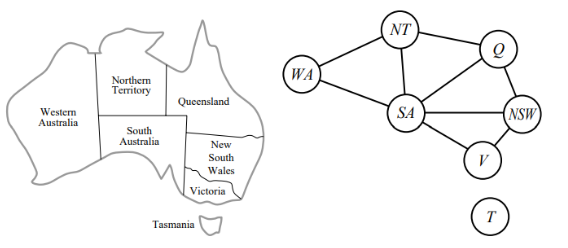
\includegraphics[width=10cm, keepaspectratio]{img/Cap1/map-coloring1.png}
    \caption{Map-Coloring}
\end{figure}
\begin{figure}[H]
    \centering
    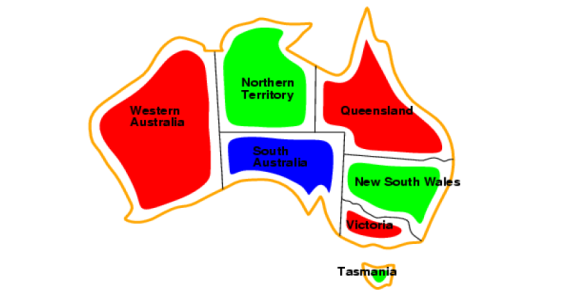
\includegraphics[width=10cm, keepaspectratio]{img/Cap1/map-coloring2.png}
    \caption{Soluzione Map-Coloring}
\end{figure}

\noindent In un CSP binario ogni vincolo è in relazione con due variabili. Il
tipo più semplice di CSP coinvolge variabili che sono discrete e hanno domini
finiti, i problemi di colorazione della mappa sono di questo tipo.

\subsection{Tipi di Variabili}
Le variabili \textbf{discrete} possono avere domini:
\begin{itemize}
    \item \textbf{Finiti:} grandezza dell'assegnamento completo $d \rightarrow
              O(d^n)$;
    \item \textbf{Infiniti:}
          \begin{itemize}
              \item hanno bisogno di un linguaggio di vincoli
              \item i vincoli lineari sono risolvibili, i non lineari sono
                    indecidibili;
          \end{itemize}
\end{itemize}
Le variabili \textbf{continue}:
\begin{itemize}
    \item Tempo di inizio e fine per specifici problemi (Hubble telescope)
\end{itemize}
Le variabili continue con dei vincoli lineari sono risolvibili in un tempo
polinomiale dai metodi LP.

\subsection{Tipi di vincoli}
\begin{itemize}
    \item \textbf{Unari:} I vincoli coinvolgono una singola variabile. $SA \neq
              green$
    \item \textbf{Binari:} I vincoli coinvolgono coppie di variabili. SA $\neq$
          W A
    \item \textbf{High order:} I vincoli coinvolgono tre o più variabili.
    \item \textbf{Preferences:} Ho una preferenza su un valore piuttosto che un
          altro per una certa variabile. Questi sono anche chiamati vincoli Soft, che
          rappresentano un costo per ogni $assegnamento$ di variabile.
\end{itemize}
Inoltre i vincoli possono essere espressi in maniera:
\begin{itemize}
    \item \textbf{Implicita:} non viene direttamente indicata la relazione fra
          gli elementi del dominio che sono permessi. Un esempio può essere $x<y$, dove
          non si elencano tutti i possibili assegnamenti delle variabili che non
          violano quel vincolo ma si possono calcolare;
    \item \textbf{Esplicita:} si elencano tutti i valori ammessi per le
          variabili coinvolte nel vincolo.
\end{itemize}
Nell'esempio precedente si avranno tutte le coppie di valori ammessi in base a
quel vincolo.

\subsection{Proprietà dei CSP}
\begin{enumerate}
    \item \textbf{Commutatività:} Si considera l'assegnamento di una singola
          variabile per volta.
    \item \textbf{Monotonicità:} Appena un vincolo viene violato posso
          interrompere la ricerca perché sono sicuro che non esisterà soluzione.
    \item \textbf{L'ordine} con il quale seleziono le variabili e assegno i
          valori è molto importante, abbiamo bisogno di euristiche intelligenti.
    \item \textbf{Indipendenza:} quando le variabili non hanno vincoli tra di
          loro (come ad esempio sulla mappa dell'Australia c'era la T che non era
          collegata agli altri nodi), il problema si può decomporre in sotto problemi
          che possono essere risolti in modo indipendente.
    \item É applicabile un controllo per \textbf{consistenza:} Invece di fare un
          controllo di consistenza alla fine, lo faccio ad ogni passo.
    \item Possono essere visti come un problema di ricerca.
\end{enumerate}

\subsection{Standard search formulation}
Gli stati sono definiti dal valore assegnato finora:
\begin{itemize}
    \item \textbf{Stato iniziale: }assegnamento vuoto \{\};
    \item \textbf{Funzione successore: }assegna un valore a una variabile non
          assegnata che non va in conflitto con l'assegnamento corrente;
    \item \textbf{Goal test: }l'assegnamento corrente è completo. Questa formula
          viene usata per tutti i CSP e ogni soluzione appare a profondità n con n
          variabili. Il cammino è irrilevante, così che può usare la formulazione
          complete-state.
\end{itemize}

\section{Metodi di ricerca sistematici}
I CSP sono problemi combinatori, quindi si deve trovare una soluzione che appartiene
all'insieme dato da tutte le possibili combinazioni di assegnamenti.
I vari metodi per fare questo sono:
\begin{enumerate}
    \item \textbf{Generate and Test: }Probabilmente il metodo di risoluzione dei
          problemi più generale. L'algoritmo consiste nei seguenti due passaggi che si
          ripetono:
          \begin{enumerate}
              \item si generano le etichette
              \item si controlla se vanno bene gli assegnamenti.
          \end{enumerate}
          Alcuni possibili miglioramenti sono ad esempio uno smart generator,
          ovvero si assegnano i valori alle variabili e se non vanno bene si
          effettuano dei cambiamenti sugli assegnamenti errati (\textbf{ricerca locale}).
          Un altro miglioramento consiste nel fare il test sugli assegnamenti e
          poi fare backtracking.
    \item \textbf{Backtracking:} Assegno uno alla volta i valori alle variabili
          finché non violo un vincolo; appena lo violo, torno indietro
          nell'assegnamento. Si estende quindi una soluzione parziale verso una
          soluzione completa.
\end{enumerate}


\subsection{Backtracking nel dettaglio}
Supponiamo di avere un problema CSP con 4 variabili $(A,B,C,D)$, supponiamo che i
vincoli siano
\begin{center}
    $A = D, B \neq D, A + C < 4$
\end{center}
L'algoritmo consiste in:
\begin{enumerate}
    \item Assegna il valore alla variabile;
    \item Si controlla la consistenza;
    \item Finché tutte le variabili sono etichettate;
\end{enumerate}

\begin{figure}[H]
    \centering
    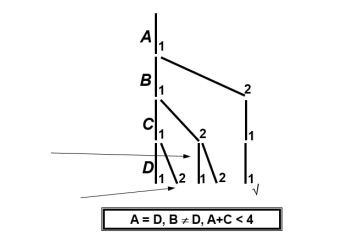
\includegraphics[width=11cm, keepaspectratio]{img/Cap2/back1.png}
    \caption{Esempio backtracking}
\end{figure}

Se tutte le variabili non sono etichettate si torna al passo 1. L'assegnamento
delle variabili è commutativo, ad esempio
\begin{center}
    $[WA = red$ allora $NT = green]$ come [$NT=green$ allora $WA =red]$
\end{center}


Si devono solo considerare gli assegnamenti alle singole variabili per ogni nodo
$\rightarrow$ b = d e ci sono $d^n$ foglie. \\La \textbf{DFS} per i CSP son gli
assegnamenti a variabili singole è chiamata ricerca \textbf{backtracking}, essa
è l'algoritmo base uniformed per i CSP.

\begin{figure}[H]
    \centering
    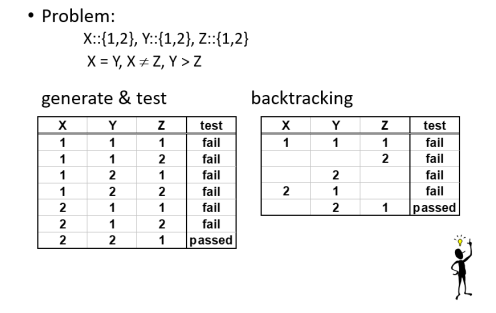
\includegraphics[width=10cm, keepaspectratio]{img/Cap2/back2.png}
    \caption{Esempio generate and test vs backtracking}
\end{figure}

\subsubsection{Ricerca backtracking: incrementale}
La strategia di ricerca è la \textbf{DFS (Depth First Search):}
\begin{enumerate}
    \item scegli una variabile non istanziata, scegli un valore dal suo dominio,
          controlla se qualche vincolo è violato;
    \item se nessun vincolo viene violato, continua la ricerca in modo
          ricorsivo;
    \item altrimenti, torna indietro: torna alla decisione precedente e fai
          un'altra scelta.
\end{enumerate}
In termini di grandezza dell'albero di ricerca il numero di foglie è pari a
$d^n$, dove n è il numero di variabili e $d = max|D_i|$.

% TODO: queste immagini vengono mostrate a cazzo su una pagina a parte 🤔
\begin{figure}[H]
    \centering
    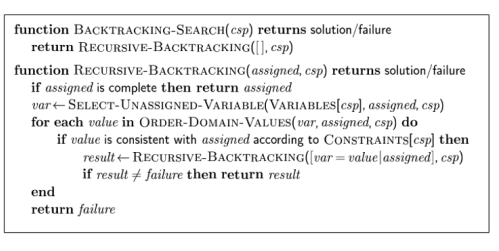
\includegraphics[width=11cm, keepaspectratio]{img/Cap2/dfs.png}
    \caption{Algoritmo di backtracking.}
\end{figure}
\begin{figure}[H]
    \centering
    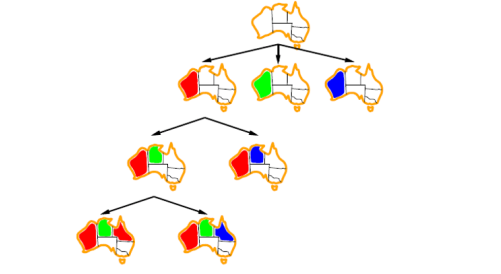
\includegraphics[width=12cm, keepaspectratio]{img/Cap2/dfs2.png}
    \caption{Esempio backtracking.}
\end{figure}

\subsection{Miglioramenti dell'efficienza del backtracking}
Per impostazione predefinita, SELECT-UNASSIGNED-VARIABLE seleziona semplicemente
la successiva variabile non assegnata nell'ordine dato dalla lista
VARIABLES[csp]. \\Questo ordinamento di variabili statiche raramente si traduce
nella ricerca più efficiente. Ad esempio, dopo le assegnazioni per WA = rosso e
NT = verde, c'è un solo valore possibile per SA, quindi ha senso assegnare SA =
blue next piuttosto che assegnare Q. Infatti, dopo l'assegnazione di SA, le
scelte per Q, NSW e V sono tutte forzate.\\

\textbf{Variabile più vincolata.} Con questo approccio si va a scegliere, fra le
variabili disponibili per l'assegnamento, quella più vincolata in base ad alcune
caratteristiche:
\begin{itemize}
    \item si sceglie la variabile con il \textbf{minor numero di valori legali}
          (\textit{minimum remaining values-MRV}). È stata anche chiamata la "variabile più
          vincolata" o euristica "fail-first", quest'ultima perché seleziona una
          variabile che ha maggiori probabilità di causare un errore presto, potando
          così l'albero di ricerca.
          \begin{figure}[H]
              \centering
              
\includegraphics[width=12cm, keepaspectratio]{img/Cap2/m1.png}
          \end{figure}
    \item si sceglie la variabile con \textbf{più vincoli possibili} (\textit{degree
              heuristic}) sulle variabili rimanenti.
          \begin{figure}[H]
              \centering
              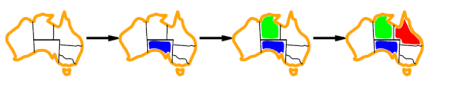
\includegraphics[width=12cm, keepaspectratio]{img/Cap2/m2.png}
          \end{figure}
    \item data una variabile, si sceglie \textbf{il valore meno vincolante}
          (\textit{least-constraining-value}), quello che esclude il minor numero di valori
          nelle restanti variabili.
          \begin{figure}[H]
              \centering
              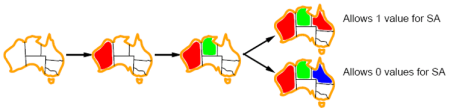
\includegraphics[width=12cm, keepaspectratio]{img/Cap2/m3.png}
          \end{figure}
\end{itemize}

\subsection{Propagazione delle informazioni attraverso vincoli}
Finora il nostro algoritmo di ricerca considera i vincoli su una variabile solo
nel momento in cui la variabile viene scelta da SELECT-UNASSIGNED-VARIABLE. Ma
guardando alcuni dei vincoli all'inizio della ricerca, o anche prima dell'inizio
della ricerca, possiamo drasticamente ridurre lo spazio di ricerca.
\subsubsection{Forward Checking}
Prima di assegnare una variabile controlla che
questo assegnamento mi renda possibile futuri assegnamenti ad altri nodi, poiché
se dopo l'assegnamento, un dominio per una variabile diventasse vuoto, non si
avrebbe soluzione e quindi l'assegnamento non andrebbe nemmeno provato.\\
\textbf{Euristica utilizzata:} elimina i valori dal dominio quando viene
fatto un assegnamento ad una variabile, \textbf{se un dominio diventa vuoto,
    interrompi la ricerca poiché la soluzione non esiste con gli assegnamenti
    fatti}. Questo metodo offre spesso una soluzione senza avere backtrack.
\begin{figure}[H]
    \centering
    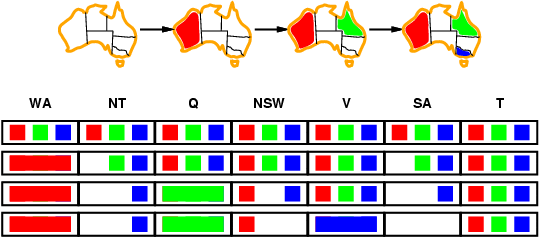
\includegraphics[width=12cm, keepaspectratio]{img/Cap2/forwod1.png}
\end{figure}
\begin{figure}[H]
    \centering
    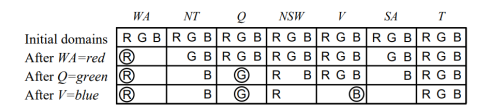
\includegraphics[width=11cm, keepaspectratio]{img/Cap2/f2.png}
    \caption{Forward checking applicata a Map-coloring problem.}
\end{figure}

In questo caso assegnare blu a V rende possibili zero colori per SA, quindi
questo tipo di assegnamento non può andare bene.
\subsubsection{Constraint propagation}
Sebbene il forward checking rilevi molte incoerenze, non le rileva tutte. Per
esempio, consideriamo la terza riga della Figura 2.5. Essa mostra che quando WA
è rosso e Q è verde, sia NT che SA sono costretti a essere blu ma questo non è
possibile perché sono due zone vicine. Il forward checking non rileva questo
come un'incoerenza, perché non guarda abbastanza avanti. La propagazione del
vincolo (constraint propagation) è il termine generale per propagare le
implicazioni di un vincolo su una variabile su altre variabili; in questo caso
dobbiamo propagare da WA e Q su NT e SA, e quindi sul vincolo tra NT e SA per
rilevare l'incoerenza.

\begin{figure}[H]
    \centering
    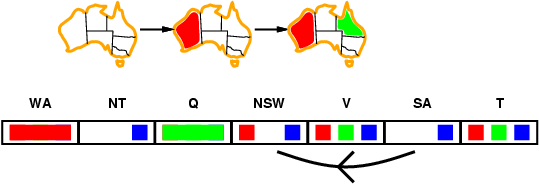
\includegraphics[width=9cm, keepaspectratio]{img/Cap3/prova4.png}
\end{figure}
\begin{figure}[H]
    \centering
    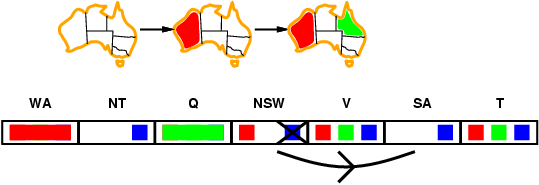
\includegraphics[width=9cm, keepaspectratio]{img/Cap3/prova5.png}
\end{figure}
\begin{figure}[H]
    \centering
    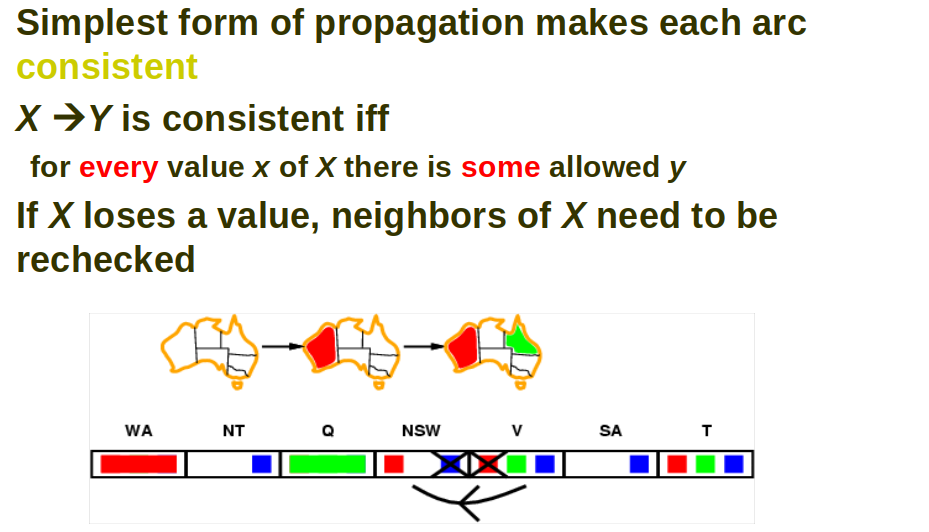
\includegraphics[width=9cm, keepaspectratio]{img/Cap3/prova6.png}
\end{figure}
\begin{figure}[H]
    \centering
    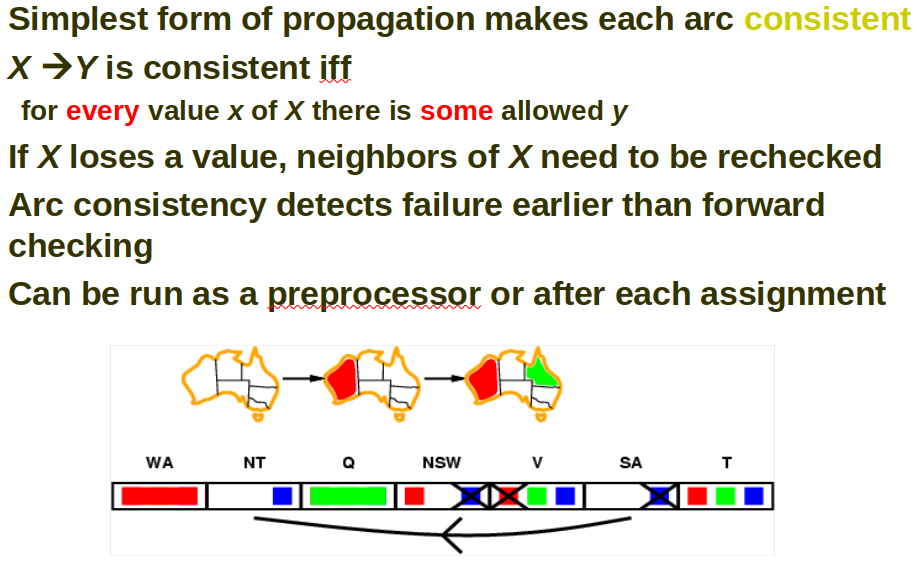
\includegraphics[width=9cm, keepaspectratio]{img/Cap3/prova7.png}
\end{figure}

\section{Local Consistency nei CSP}
\textbf{La consistenza locale} è la condizione che si verifica quando ogni nodo
di una rete soddisfa tutti i vincoli che lo coinvolgono. Quest'ultima nei CSP
consente di \textbf{ridurre lo spazio di ricerca} di un algoritmo eliminando dal
dominio delle variabili i valori che non rispettano i vincoli, cioè che non
hanno \textbf{supporto}; può essere definita in rapporto alla consistenza di
nodo, arco o cammino.
\begin{itemize}
    \item \textbf{Consistenza di Nodo:} Consiste nella verifica dei valori del
          dominio di un nodo rispetto ai vincoli del nodo stesso. Ad esempio, se il
          dominio del nodo $x_1$ è pari a \{$1,2,3$\} e il vincolo unario di $x_1$ è $x_1 >
              1$, la consistenza di nodo consente di ridurre il dominio di $x_1$ a \{$2,3$\}
          riducendo il processo di ricerca dell'algoritmo.
    \item \textbf{Consistenza di Arco:} Consiste nella verifica dei valori di un
          dominio di un nodo rispetto ai vincoli binari con un altro nodo. Ad esempio,
          dati due nodi $x_1$ e $x_2$ con rispettivi domini \{$1,2,3$\} e \{$1,4,5,9$\}, il
          vincolo $x_2 = x_{1}^2$ consente di ridurre il dominio del nodo $x_2$ a \{$1,4,9$\}
          poiché non sussiste alcun nesso tra il valore 5 dell'insieme dominio di
          $x_2$ e qualsiasi altro elementi dell'insieme dominio di $x_1$.
    \item \textbf{Consistenza di Cammino:} Consiste nella verifica dei valori di
          un nodo rispetto ai vincoli n-ari con altri n nodi. La consistenza di
          cammino è un estensione della consistenza di arco ed è detta anche
          k-consistenza. Si distingue dalla consistenza di arco che, invece, è
          dedicata ai vincoli binari tra due nodi.
\end{itemize}

\subsection{Node Consistency}
In questo caso tutti i vincoli sono unari, le variabili sono rappresentate da
dei \textbf{vertici}. Il vertice è \textbf{node consistent} se ogni valore nel
dominio delle variabili soddisfa tutti i vincoli unari imposti sulla variabile
X. Spesso vengono rappresentati come un cappio o arco che ritorna sullo stesso
nodo.

\begin{figure}[H]
    \centering
    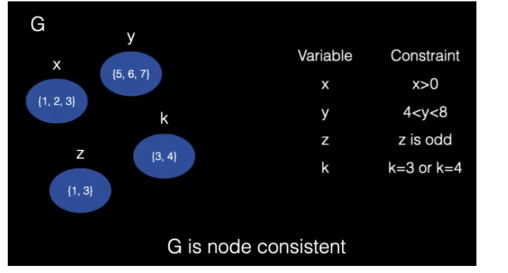
\includegraphics[width=10cm, keepaspectratio]{img/Cap3/node1.png}
    \caption{Esempio grafo node consistent}
\end{figure}

\subsection{Arc Consistency}
Quando tutti i vincoli sono binari si parla di arc consistency. Un arco $(u,v)$ è
consistente se per ogni valore $x$ del dominio $dom(u)$ esiste un valore $y$ nel
$dom(v)$ tale che un assegnamento $u=x$ e $v=y$ soddisfa tutti i vincoli binari
che coinvolgono sia $u$ che $v$.

\paragraph{Punto fisso e supporto:}
Tutto il processo di consistenza locale viene applicato fin quando non si riesce
a trovare un punto fisso, cioè fino a quando il dominio delle variabili resta
invariato.

\paragraph{Problema arc-consistente:} Un problema nel quale applicando local
consistency, nessun dominio di nessuna variabile viene modificato.

\paragraph{Supporto:} Per la riduzione dobbiamo vedere quali elementi
hanno supporto in Y, ovvero quali hanno un assegnamento in Y tale per cui il
vincolo viene soddisfatto.

\begin{figure}[H]
    \centering
    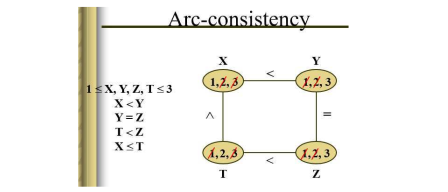
\includegraphics[width=13cm, keepaspectratio]{img/Cap3/esempio-arc.png}
    \caption{Esempio arc-consistency}
\end{figure}


Quando $X=1$ esiste un elemento in Y tale per cui $X < Y$? Si, 2,3\\
Quando $X=2$ esiste un elemento in Y tale per cui $X < Y$? Si, 3\\
Quando $X=3$ esiste un elemento in Y tale per cui $X < Y$?\\
No, quindi posso eliminare 3 il dominio di X\\

L'operazione che ho fatto si chiama Local Consistency, ma dato che ho utilizzato
il vincolo binario si chiama Arc Consistency.\\

\paragraph{Conclusione:} In questo caso sono stato molto fortunato perché
è rimasto 1 solo valore possibile per ogni variabile. Quindi la soluzione è
unica e sarà:

$$
    X = 1, Y = 3, Z = 3, T = 2
$$

Se fossi stato meno fortunato comunque avrei ridotto gli elementi del dominio e
quindi quando sarei andato a fare la ricerca con backtrack comunque lo spazio di
ricerca si sarebbe di molto diminuito (avrei controllano meno assegnamenti).

\paragraph{Vantaggio dell'applicazione della Local Consistency prima della Backtracking:}
Se faccio backtrack il dominio degli stati che
vado ad esplorare è esponenziale perché ad X dovrei moltiplicare tutti i
possibili valori di Y, a cui dovrei moltiplicare tutti i possibili valori di Z
che moltiplico per tutti i valori possibili per T. All'inizio quindi in quel
problema si avevano $3^4 = 81$ possibili assegnamenti, mentre se applico prima
Local Consistency il problema diventa polinomiale (facile) rispetto al numero di
variabili che coinvolgo (in questo caso lo spazio di ricerca mi si riduce ad 1).

\subsection{Algoritmi per Consistenza Locale}
\subsubsection{Procedura Revise}
Per fare diventare un arco $(u,v)$ consistente si cancellano tutti i valori $x$ dal
$dom(u)$ che sono inconsistenti con tutti i valori in $dom(v)$. \\Restituisce true se
è stata fatta una modifica al dominio di $u$.
\begin{figure}[H]
    \centering
    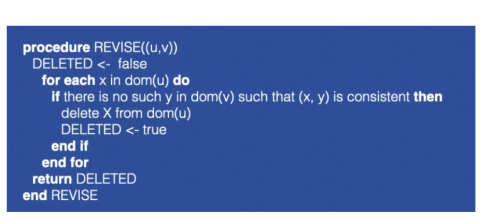
\includegraphics[width=13cm, keepaspectratio]{img/Cap3/revise.png}
    \caption{Procedura REVISE}
\end{figure}

\subsubsection{Algoritmo AC-1}
Un singolo passo dell'algoritmo REVISE non è sufficiente. L'algoritmo base per
arc consistency è AC-1, il quale esegue l'algoritmo REVISE finché il dominio
delle variabili cambia. In questo si ripete la procedura REVISE ogni volta che
viene modificato un valore in un dominio.

\begin{figure}[H]
    \centering
    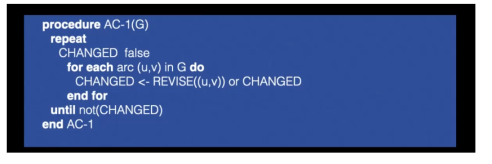
\includegraphics[width=13cm, keepaspectratio]{img/Cap3/ac-1.png}
    \caption{Algoritmo AC-1}
\end{figure}

Una sola revisione riuscita di un arco su una particolare iterazione causa la
revisione di tutti gli archi nella prossima iterazione anche se gli archi non
sono influenzati dal cambiamento.\\
\textbf{L'inefficienza} sta nel fatto che se anche una singola chiamata alla
procedura di REVISE su una particolare iterazione risultasse vera, tutti gli
archi verrebbero scansionati nuovamente nella successiva iterazione. Questo però
non è sempre necessario, perché la modifica del dominio di una variabile
influenza solamente le variabili che sono collegate a X da un vincolo e non le
restanti.\\
La complessità temporale è $O(e \cdot n \cdot d^3)$ e quella spaziale è $O(e \cdot n \cdot d)$.

\subsubsection{Algoritmo AC-2}
AC-2 è un algoritmo che può fare arc consistency in un solo passo attraverso i
nodi. Il risultato è ottenuto passando per i nodi in un ordine numerico:
\begin{itemize}
    \item Allegare ad un nodo tutti i valori che non sono in conflitto con i
          nodi precedentemente assegnati;
    \item Guarda i vicini di questo nodo che sono stati già valutati; se un
          valore non ha un'assegnazione corrispondente per lo stesso arco, eliminalo;
    \item Ogni volta che qualsiasi valore è cancellato da un arco, guarda ai
          suoi vicini a sua volta, e controlla se un loro valore può essere eliminato.
          Se può essere eliminato, si continua il processo iterativamente finché non
          ci sono più cambiamenti che possono essere fatti. Poi si prosegue con gli
          altri archi.
\end{itemize}
In sostanza si sceglie un ordine fra i nodi, prendiamo ad esempio y come primo e
controlliamo tutti i vincoli fra $y$ e $k$ se c'è qualche valore di $dom(y)$ che va in
conflitto allora si elimina. Stessa cosa si per l'arco $(x,y)$ se si fa qualche
modifica si rimette in coda l'arco in modo da controllare se ci sono altre
modifiche da fare. Se un valore $b$ del nodo $i$ è rimosso allora si aggiunge tutti
$(k,i)$ alla coda Q, per il controllo degli archi.

\begin{figure}[H]
    \centering
    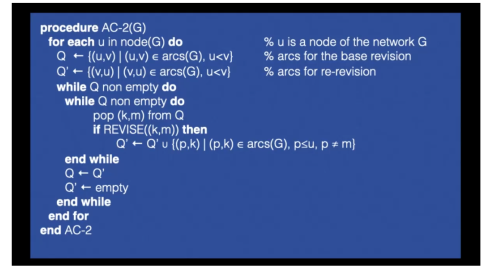
\includegraphics[width=13cm, keepaspectratio]{img/Cap3/ac-2.png}
    \caption{Algoritmo AC-2}
\end{figure}

La complessità temporale è $O(n^2 \cdot d^3)$ e quella spaziale è $O(n^2$).

\subsubsection{Algoritmo AC-3}
AC-3 è un miglioramento di AC-2, alcuni di essi possono essere già nella
coda Q. Se è così allora non dovrebbero essere inseriti di nuovo.

\begin{figure}[H]
    \centering
    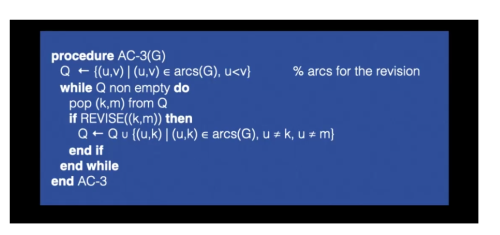
\includegraphics[width=13cm, keepaspectratio]{img/Cap3/ac-3.png}
    \caption{Algoritmo AC-3}
\end{figure}

In sostanza si prende un arco dalla coda Q, si fa la REVISE, se faccio una
modifica allora si aggiunge alla coda Q tutti gli archi $(u,k)$ che non sono stati
già controllati ovvero $u \neq k$ e $u \neq m$.\\
La complessità temporale è $O(n^2 \cdot d^2)$ e quella spaziale è $O(n^2$).

\section{Ricapitolando}

\subsection{Arc-consistency}

Algoritmo che ha la caratteristica di lavorare a livello locale sul CSP.
L'obiettivo è quello di semplificarlo in maniera tale da ridurre la quantità di
elementi possibili nel dominio e quindi ridurre il tempo necessario quando
faccio la ricerca con backtrack. \\\textbf{Supporto: } un elemento del dominio
di X può essere buttato via se non ha supporto in y.
\begin{figure}[H]
    \centering
    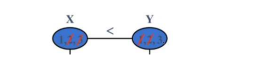
\includegraphics[width=9cm, keepaspectratio]{img/Cap3/riassunto1.png}
\end{figure}

Ad esempio, 1 ha supporto in X perché in Y c'è 2 e 3. Se un elemento non ha
supporto lo posso escludere dai valori assegnabili alla variabile. Un problema
si dice arc-consistente se ho buttato via tutti gli elementi che NON hanno
supporto.

\vspace{0.8cm}

\textbf{Questo è un problema Arc-Consistente?}
\begin{figure}[H]
    \centering
    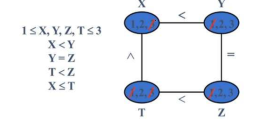
\includegraphics[width=9cm, keepaspectratio]{img/Cap3/riassunto2.png}
\end{figure}

No, perché il 2 andrebbe eliminato da Z. Se riesco a buttare via tutti gli
elementi che non hanno supporto allora il problema diventa arc-consistente.

\subsection{Soluzione di un CSP}
La soluzione ad un problema è un assegnamento per tutte le variabili. \\Nel caso
in cui fossi interessato solo ad un sottoinsieme di variabili parliamo di
\textbf{Vincolo Distinto.} Le operazioni sono:
\begin{itemize}
    \item  \textbf{Combinazione} tra i vincoli.
    \item \textbf{Proiezione} nel caso in cui esista questo vincolo distinto.
\end{itemize}
Queste operazioni sono di tipo insiemistico nel caso dei CSP classici (Crisp),
nel caso in cui invece passiamo a dei problemi di vincoli Soft, e quindi è
presente una nozione di priorità tra le soluzioni (il rosso mi costa più del
giallo) parliamo di SCSP.

\subsection{Applicare Local Consistency durante il Backtrack}
L'esempio fatto adesso applica la Local Consistency prima di fare Backtrack.
Tuttavia è possibile applicarla anche durante la ricerca con backtrack ogni
volta che si modifica il dominio di una variabile, vediamo come: (credo che
serva solamente sapere che si può fare anche durante e non l'esempio vero e
proprio).
\begin{figure}[H]
    \centering
    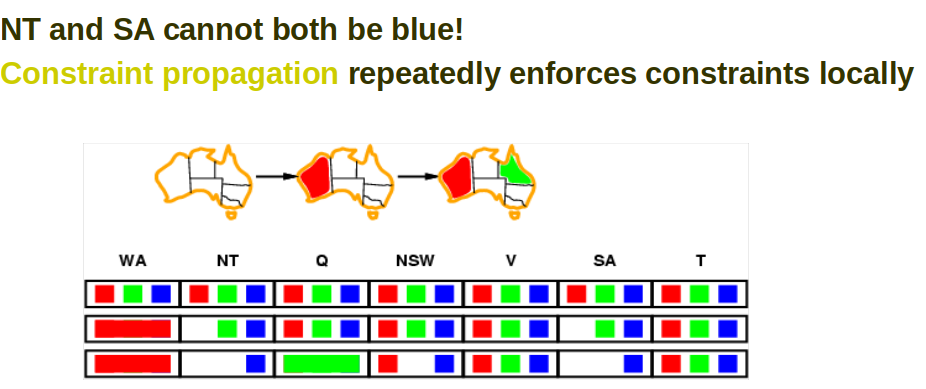
\includegraphics[width=12cm, keepaspectratio]{img/Cap3/prova3.png}
\end{figure}

\subsubsection{L'Arc Consistency è sufficiente ?}
Se ci dice bene si, come visto sopra (tolgo talmente tante cose che la soluzione
me la trova da solo), ma la maggior parte delle volte permette solamente di
restringere lo spazio di ricerca, quindi si può rendere un CSP arc-consistente e
poi cercare una soluzione con backtracking; oppure assegnare iterativamente un
valore e rendere le variabili restanti arco consistenti. Inoltre, se il dominio
di una variabile diventa vuoto, sappiamo che non esisterà soluzione.

\subsection{Vincolo distinto (Proiezione)}
Alcune volte non ci interessa sapere il valore che possono ottenere tutte le
variabili, ma solamente un sottoinsieme di esse. Definiamo quindi il: \\
\textbf{Vincolo distinto (proiezione):} Quali sono gli elementi del problema di
cui vogliamo conoscere la soluzione.

